\documentclass[12pt,a4paper]{article}

% Encoding and fonts
\usepackage[utf8]{inputenc}
\usepackage[T1]{fontenc}
\usepackage{lmodern}

% Page layout
\usepackage[margin=2.5cm]{geometry}
\usepackage{setspace}
\usepackage{parskip}

% Colors and graphics
\usepackage[dvipsnames,svgnames]{xcolor}
\usepackage{tikz}
\usetikzlibrary{calc,positioning,decorations.pathmorphing}

% Tables and lists
\usepackage{booktabs}
\usepackage{array}

% Headers and formatting
\usepackage{fancyhdr}
\usepackage{titlesec}
\usepackage{hyperref}
\usepackage{enumitem}

% Define colors
\definecolor{udeaverde}{RGB}{0,105,56}
\definecolor{udeaazul}{RGB}{0,62,115}
\definecolor{accent}{RGB}{34,113,73}
\definecolor{tierra}{RGB}{139,90,43}
\definecolor{cielo}{RGB}{135,190,220}
\definecolor{bosque}{RGB}{46,125,50}
\definecolor{gris}{RGB}{90,90,90}
\definecolor{segura}{RGB}{46,125,50}
\definecolor{riesgo}{RGB}{201,143,30}
\definecolor{alto}{RGB}{183,55,55}

% Hyperref setup
\hypersetup{
  colorlinks=true,
  linkcolor=udeaazul,
  citecolor=udeaazul,
  urlcolor=udeaazul
}

% Header/footer style
\pagestyle{fancy}
\fancyhf{}
\fancyhead[L]{\small\color{gris}\textit{C\'{a}tedra Ambiental -- L\'{i}mites planetarios}}
\fancyhead[R]{\small\color{gris}\textit{Universidad de Antioquia}}
\fancyfoot[C]{\small\color{gris}\thepage}
\renewcommand{\headrulewidth}{0.4pt}
\renewcommand{\headrule}{\hbox to\headwidth{\color{udeaverde}\leaders\hrule height \headrulewidth\hfill}}

% Section formatting
\titleformat{\section}
  {\Large\bfseries\color{udeaazul}}
  {}{0em}{}
\titleformat{\subsection}
  {\large\bfseries\color{accent}}
  {}{0em}{}

% Helper command for a colored zone tag
\newcommand{\zona}[2]{\textcolor{#1}{\textbf{#2}}}

\begin{document}

% ============================================================
% COVER PAGE
% ============================================================
\thispagestyle{empty}

\begin{tikzpicture}[remember picture, overlay]

  %  Background gradient block (top)
  \fill[udeaazul] (current page.north west) rectangle ([yshift=-8cm]current page.north east);

  % Decorative wave at bottom of blue block
  \fill[white, decoration={snake, amplitude=2mm, segment length=20mm}, decorate]
    ([yshift=-7.8cm]current page.north west) -- ([yshift=-7.8cm]current page.north east)
    -- ([yshift=-8.5cm]current page.north east) -- ([yshift=-8.5cm]current page.north west) -- cycle;
  \fill[white] ([yshift=-8.5cm]current page.north west) rectangle (current page.south east);

  %  Green accent stripe
  \fill[udeaverde] ([yshift=-8.2cm]current page.north west) rectangle ([yshift=-8.6cm]current page.north east);

  %  University name
  \node[anchor=north, text=white, font=\fontsize{11}{13}\selectfont\scshape]
    at ([yshift=-1.2cm]current page.north) {Universidad de Antioquia};
  \node[anchor=north, text=cielo, font=\fontsize{9}{11}\selectfont]
    at ([yshift=-1.9cm]current page.north) {Videojuego educativo interactivo};

  %  Title block
  \node[anchor=center, text=white, font=\fontsize{30}{36}\selectfont\bfseries, text width=14cm, align=center]
    at ([yshift=-4.2cm]current page.north) {Guardianes del Holoceno};
  \node[anchor=center, text=cielo, font=\fontsize{16}{20}\selectfont\itshape, text width=14cm, align=center]
    at ([yshift=-5.8cm]current page.north) {Un videojuego sobre los nueve l\'{i}mites planetarios};

  %  Decorative icons (simple)
  \node[anchor=center, text=white, opacity=0.15, font=\fontsize{80}{80}\selectfont]
    at ([xshift=-6cm, yshift=-3cm]current page.north) {\textbf{\&}};
  \node[anchor=center, text=white, opacity=0.12, font=\fontsize{60}{60}\selectfont, rotate=25]
    at ([xshift=6.5cm, yshift=-6cm]current page.north) {\textbf{@}};

  %  Course and module
  \node[anchor=north, font=\fontsize{14}{17}\selectfont\bfseries, text=udeaverde]
    at ([yshift=-9.8cm]current page.north) {C\'{a}tedra Ambiental};
  \node[anchor=north, font=\fontsize{11}{13}\selectfont, text=gris]
    at ([yshift=-10.6cm]current page.north) {Evaluaci\'{o}n M\'{o}dulo 4 \textbullet{} L\'{i}mites planetarios};

  %  Decorative line
  \draw[udeaverde, line width=1.2pt]
    ([xshift=5cm, yshift=-11.4cm]current page.north west) -- ([xshift=-5cm, yshift=-11.4cm]current page.north east);

  %  Author info block
  \node[anchor=north, text width=12cm, align=center] at ([yshift=-12.4cm]current page.north) {
    {\fontsize{14}{18}\selectfont\color{udeaazul}\textbf{Johan Granados Vega}}\\[6pt]
    {\fontsize{11}{14}\selectfont\color{gris} Estudiante del Programa de Estad\'{i}stica}\\[3pt]
    {\fontsize{11}{14}\selectfont\color{gris} Facultad de Ciencias Exactas y Naturales}\\[3pt]
    {\fontsize{11}{14}\selectfont\color{gris} Universidad de Antioquia}
  };

  %  Professor info
  \node[anchor=north, text width=12cm, align=center] at ([yshift=-16cm]current page.north) {
    {\fontsize{10}{13}\selectfont\color{gris} Trabajo presentado a:}\\[4pt]
    {\fontsize{12}{15}\selectfont\color{accent}\textbf{Profesora Cristina L\'{o}pez-Gallego}}\\[3pt]
    {\fontsize{10}{13}\selectfont\color{gris} Curso: C\'{a}tedra Ambiental}
  };

  %  Decorative green bottom bar
  \fill[udeaverde] ([yshift=1.5cm]current page.south west) rectangle ([yshift=1.9cm]current page.south east);
  \fill[udeaazul] ([yshift=0cm]current page.south west) rectangle ([yshift=1.5cm]current page.south east);

  %  Date
  \node[anchor=center, text=white, font=\fontsize{11}{13}\selectfont]
    at ([yshift=0.75cm]current page.south) {Medell\'{i}n, 2026};

\end{tikzpicture}

\newpage

% ============================================================
% BODY
% ============================================================
\setstretch{1.5}

\section*{Introducci\'{o}n}

\vspace{0.3cm}

Durante aproximadamente 11.700 a\~{n}os, el Holoceno le ofreci\'{o} a la humanidad un planeta excepcionalmente estable: un clima predecible, ecosistemas resilientes y ciclos biogeoqu\'{i}micos en equilibrio que hicieron posible la agricultura, las ciudades y la civilizaci\'{o}n tal como la conocemos. En 2009, Johan Rockstr\"{o}m y los cient\'{i}ficos del Centro de Resiliencia de Estocolmo propusieron el marco de los nueve l\'{i}mites planetarios: los umbrales dentro de los cuales la humanidad puede operar con seguridad y m\'{a}s all\'{a} de los cuales el sistema terrestre corre el riesgo de cambios abruptos e irreversibles. Hoy, seis de esos nueve l\'{i}mites ya han sido transgredidos.

Comprender este marco constituye uno de los objetivos centrales del M\'{o}dulo 4 de la C\'{a}tedra Ambiental. En esa direcci\'{o}n, este trabajo propone el desarrollo de un recurso pedag\'{o}gico interactivo: el videojuego educativo \emph{Guardianes del Holoceno}. En \'{e}l, la persona que juega asume la responsabilidad de gobernar el planeta y experimenta, de manera vivencial, c\'{o}mo las decisiones colectivas pueden degradar o restaurar las condiciones que sostienen la vida en la Tierra. As\'{i}, el juego convierte los conceptos abordados en la cartilla del m\'{o}dulo los l\'{i}mites planetarios, el Antropoceno y el Capitaloceno, la cultura de los l\'{i}mites y la justicia socioambiental en mec\'{a}nicas concretas, dilemas con consecuencias y una representaci\'{o}n visual del estado del sistema terrestre.

Este documento presenta el proyecto: sus objetivos, la descripci\'{o}n detallada del interactivo y los enlaces de acceso a la versi\'{o}n desplegada en la web y al c\'{o}digo fuente abierto.

\section*{Objetivos}

\subsection*{Objetivo general}

Dise\~{n}ar y desarrollar un videojuego educativo interactivo, accesible desde la web, que comunique de forma vivencial el concepto de los nueve l\'{i}mites planetarios y los contenidos del M\'{o}dulo 4 de la C\'{a}tedra Ambiental, de modo que quien juega comprenda la interdependencia entre las decisiones humanas y la estabilidad del sistema terrestre.

\subsection*{Objetivos espec\'{i}ficos}

\begin{itemize}[leftmargin=1.4em, itemsep=4pt]
  \item Traducir los nueve l\'{i}mites planetarios definidos por Rockstr\"{o}m \textit{et al.} (2009) y actualizados por Steffen \textit{et al.} (2015), Persson \textit{et al.} (2022) y Wang-Erlandsson \textit{et al.} (2022) en variables medibles dentro de una mec\'{a}nica de juego por turnos.
  \item Representar visualmente la degradaci\'{o}n y la recuperaci\'{o}n del planeta mediante una Tierra animada y un diagrama radial que reflejan, en tiempo real, las consecuencias de cada decisi\'{o}n.
  \item Integrar \emph{pausas de saberes} (preguntas tipo quiz) que refuercen los conceptos clave de la cartilla y recompensen el aprendizaje aliviando los l\'{i}mites m\'{a}s transgredidos.
  \item Evidenciar las dimensiones de justicia socioambiental la responsabilidad diferenciada entre el Norte y el Sur global y la noci\'{o}n de Capitaloceno como parte ineludible de la crisis planetaria.
  \item Desplegar la aplicaci\'{o}n en un servidor p\'{u}blico y liberar el c\'{o}digo fuente para garantizar el acceso abierto, la reproducibilidad y el uso pedag\'{o}gico del recurso.
\end{itemize}

\section*{\textquestiondown De qu\'{e} trata? El interactivo}

\emph{Guardianes del Holoceno} es un juego de estrategia y decisi\'{o}n por turnos en el que asumes el gobierno del mundo entre los a\~{n}os 2025 y 2090. Cada turno representa un lapso de cinco a\~{n}os y plantea una decisi\'{o}n o una pregunta. La premisa es directa: el Holoceno nos regal\'{o} un planeta estable, pero seis de los nueve l\'{i}mites ya fueron transgredidos, y de tus decisiones depende devolver a la humanidad a un espacio operativo seguro o precipitar el colapso.

\subsection*{Los nueve l\'{i}mites en juego}

El estado del planeta se mide a trav\'{e}s de los nueve l\'{i}mites planetarios. Cada uno se cuantifica en una escala de transgresi\'{o}n de 0 a 100, dividida en tres zonas: \zona{segura}{zona segura} (0--32), \zona{riesgo}{zona de riesgo} (33--65) y \zona{alto}{zona de alto riesgo} (66--100). La partida comienza con el planeta ya bajo presi\'{o}n:

\begin{center}
\setstretch{1.15}
\renewcommand{\arraystretch}{1.35}
\begin{tabular}{>{\raggedright\arraybackslash}p{6.2cm} c c}
\toprule
\textbf{L\'{i}mite planetario} & \textbf{Nivel inicial} & \textbf{Zona} \\
\midrule
Ciclos de nitr\'{o}geno y f\'{o}sforo & 75 & \zona{alto}{Alto riesgo} \\
Integridad de la bi\'{o}sfera & 70 & \zona{alto}{Alto riesgo} \\
Nuevas entidades (pl\'{a}sticos) & 62 & \zona{riesgo}{Riesgo} \\
Cambio clim\'{a}tico & 55 & \zona{riesgo}{Riesgo} \\
Cambios en los sistemas de suelo & 50 & \zona{riesgo}{Riesgo} \\
Agua verde & 48 & \zona{riesgo}{Riesgo} \\
Acidificaci\'{o}n de los oc\'{e}anos & 32 & \zona{segura}{Segura} \\
Aerosoles atmosf\'{e}ricos & 28 & \zona{segura}{Segura} \\
Ozono estratosf\'{e}rico & 15 & \zona{segura}{Segura} \\
\bottomrule
\end{tabular}
\end{center}

\subsection*{C\'{o}mo se juega}

A lo largo de la partida tomas trece decisiones: diez \emph{dilemas} de gobernanza intercalados con tres \emph{pausas de saberes}. Cada dilema presenta una situaci\'{o}n real --la matriz energ\'{e}tica, alimentar al mundo, el secamiento de la Amazon\'{i}a, el planeta pl\'{a}stico, el ciclo del agua verde, las ciudades, la meta del crecimiento (PIB), la geoingenier\'{i}a, la pesca de arrastre y la negociaci\'{o}n Norte Sur global con tres opciones de respuesta. Cada opci\'{o}n modifica los niveles de los l\'{i}mites y un indicador de bienestar social, y ofrece una retroalimentaci\'{o}n que explica las consecuencias de la elecci\'{o}n a la luz de la cartilla.

Las \emph{pausas de saberes} son preguntas de opci\'{o}n m\'{u}ltiple sobre los contenidos del m\'{o}dulo (por ejemplo, cu\'{a}ntos l\'{i}mites planetarios existen, qu\'{e} significa el ``agua verde'' o qu\'{e} propone el concepto de \emph{Capitaloceno}). Si aciertas, el conocimiento ``sana'': se alivian autom\'{a}ticamente los dos l\'{i}mites m\'{a}s transgredidos. As\'{i}, el juego premia el aprendizaje como herramienta de transformaci\'{o}n.

\subsection*{La Tierra que reacciona}

El coraz\'{o}n visual del juego es una \textbf{Tierra animada que gira en pantalla} y que \textbf{sana o se marchita} con cada decisi\'{o}n: los oc\'{e}anos, los continentes, las nubes y el esmog cambian seg\'{u}n la salud planetaria. Un diagrama radial muestra simult\'{a}neamente el estado de los nueve l\'{i}mites, permitiendo ver de un vistazo cu\'{a}les est\'{a}n en zona segura, de riesgo o de alto riesgo. Esta retroalimentaci\'{o}n inmediata convierte conceptos abstractos en una experiencia tangible.

\subsection*{Finales posibles}

La partida puede terminar de forma anticipada por un colapso social (si el bienestar se desploma) o un colapso planetario (si demasiados l\'{i}mites cruzan la zona de alto riesgo). Si se completa el recorrido hasta 2090, el resultado depende del estado final del planeta: \zona{segura}{Guardiana/Guardi\'{a}n del Holoceno} (espacio seguro recuperado sin sacrificar el bienestar), \emph{Equilibrista planetario}, \emph{Al borde del abismo} o \zona{alto}{Una herencia rota}. Cada final cierra con una reflexi\'{o}n de autores como Kallis, Hamilton o Latour, conectando la experiencia de juego con el pensamiento ambiental del m\'{o}dulo.

\subsection*{C\'{o}mo est\'{a} construido}

El juego es una aplicaci\'{o}n web desarrollada en Python con el microframework Flask. El motor del juego gestiona el estado, los efectos de cada decisi\'{o}n y las condiciones de fin; el contenido (l\'{i}mites, dilemas y preguntas) se basa directamente en la cartilla ``Ciencia, conflictos y alternativas para el siglo XXI'' (Orozco-Echeverri, Mira Boh\'{o}rquez y Mu\~{n}oz Fonnegra, UdeA). La interfaz emplea HTML, CSS animado y gr\'{a}ficos SVG para el planeta y el diagrama radial. La aplicaci\'{o}n est\'{a} desplegada en la plataforma Railway y su c\'{o}digo es abierto.

\section*{Enlaces de acceso}

\begin{center}
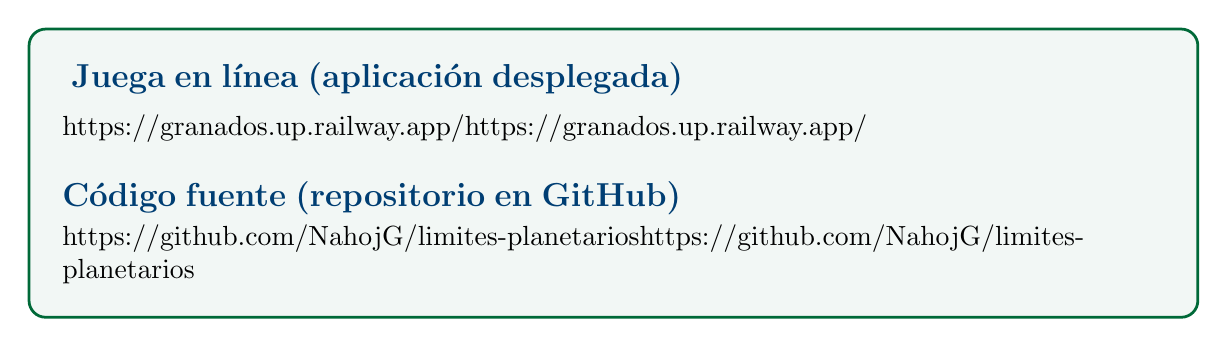
\begin{tikzpicture}
  \node[draw=udeaverde, line width=1pt, rounded corners=6pt, fill=udeaverde!5,
        inner sep=12pt, text width=14cm] {
    \setstretch{1.3}
    {\color{udeaazul}\textbf{\large Juega en l\'{i}nea (aplicaci\'{o}n desplegada)}}\\[2pt]
    \href{https://granados.up.railway.app/}{https://granados.up.railway.app/}\\[10pt]
    {\color{udeaazul}\textbf{\large C\'{o}digo fuente (repositorio en GitHub)}}\\[2pt]
    \href{https://github.com/NahojG/limites-planetarios}{https://github.com/NahojG/limites-planetarios}
  };
\end{tikzpicture}
\end{center}

\vspace{0.2cm}

El videojuego puede jugarse directamente desde cualquier navegador moderno, sin necesidad de instalaci\'{o}n, a trav\'{e}s del primer enlace. El segundo enlace da acceso al c\'{o}digo fuente completo, las instrucciones para ejecutarlo localmente y la documentaci\'{o}n del proyecto.

\vspace{1cm}





\end{document}
